\chapter{Computation of Orientation}
\label{ch:orientationcomp}
\section{Computing the orientation using Euler Angles}
\subsection{Integration of angular rate}

\indent \indent Triaxial gyroscopes measure the angular rate around each one of the Cartesian axes relative to the body frame. Such angular rate can be integrated to estimate the rotation angle from time instants $t_{0}$ to $t_{1}$. Therefore, we can compute the position of the body relative to the navigation frame if, and only if, the initial orientation of the body frame with respect to the navigation frame is known. A straight forward solution is to use the approach based on the projection of the gravity and earth's magnetic field vectors to compute such initial orientation when the body is static.\\
\indent Many different numerical integration methods can be used to integrate the angular rate. In this case we will use the numerical integration based on the trapezoidal rule which calculates the area under the function performing a trapezoidal approximation as follows:
\begin{gather}
\alpha(n)=\alpha_{0}+\frac{T}{2}\sum_{k=1}^{n}\left[\omega_{\mbox{\scriptsize g}}(k)+\omega_{\mbox{\scriptsize g}}(k-1)\right]
\label{eq:trapInt}
\end{gather}
Where T is the sample period, $n$ the sample number, $\omega_{\mbox{\scriptsize g}}(n)$ the gyro measurement at instant $n$ and $\alpha_{0}$ the angle at $n=0$. The angle can also be computed in a recursive way using
\begin{equation}
\alpha(n)=\alpha(n-1)+\frac{\mbox{T}}{2}\left[\omega_{\mbox{\scriptsize g}}(n)+\omega_{\mbox{\scriptsize g}}(n-1)\right]
\label{eq:trapIntRec}
\end{equation}
where $\alpha(0)=\alpha_{0}$.\\
\indent The main advantage of this method is that, once the initial orientation is known, it can be used either under low or high intensity motion conditions as the gyroscope measurements are not affected by linear acceleration. However, integration of noise and dynamic bias leads to a quick time growing offset which disrupts the computed angle. The effects of such integration are so devastating that the orientation estimate is absolutely erroneous after a few seconds as it can be seen in figure \ref{fig:dynBiasEff}).\\
\indent This method is, itself, unfeasible if not fused with the accelerometer and magnetometer approach. 
\begin{figure}
\centering
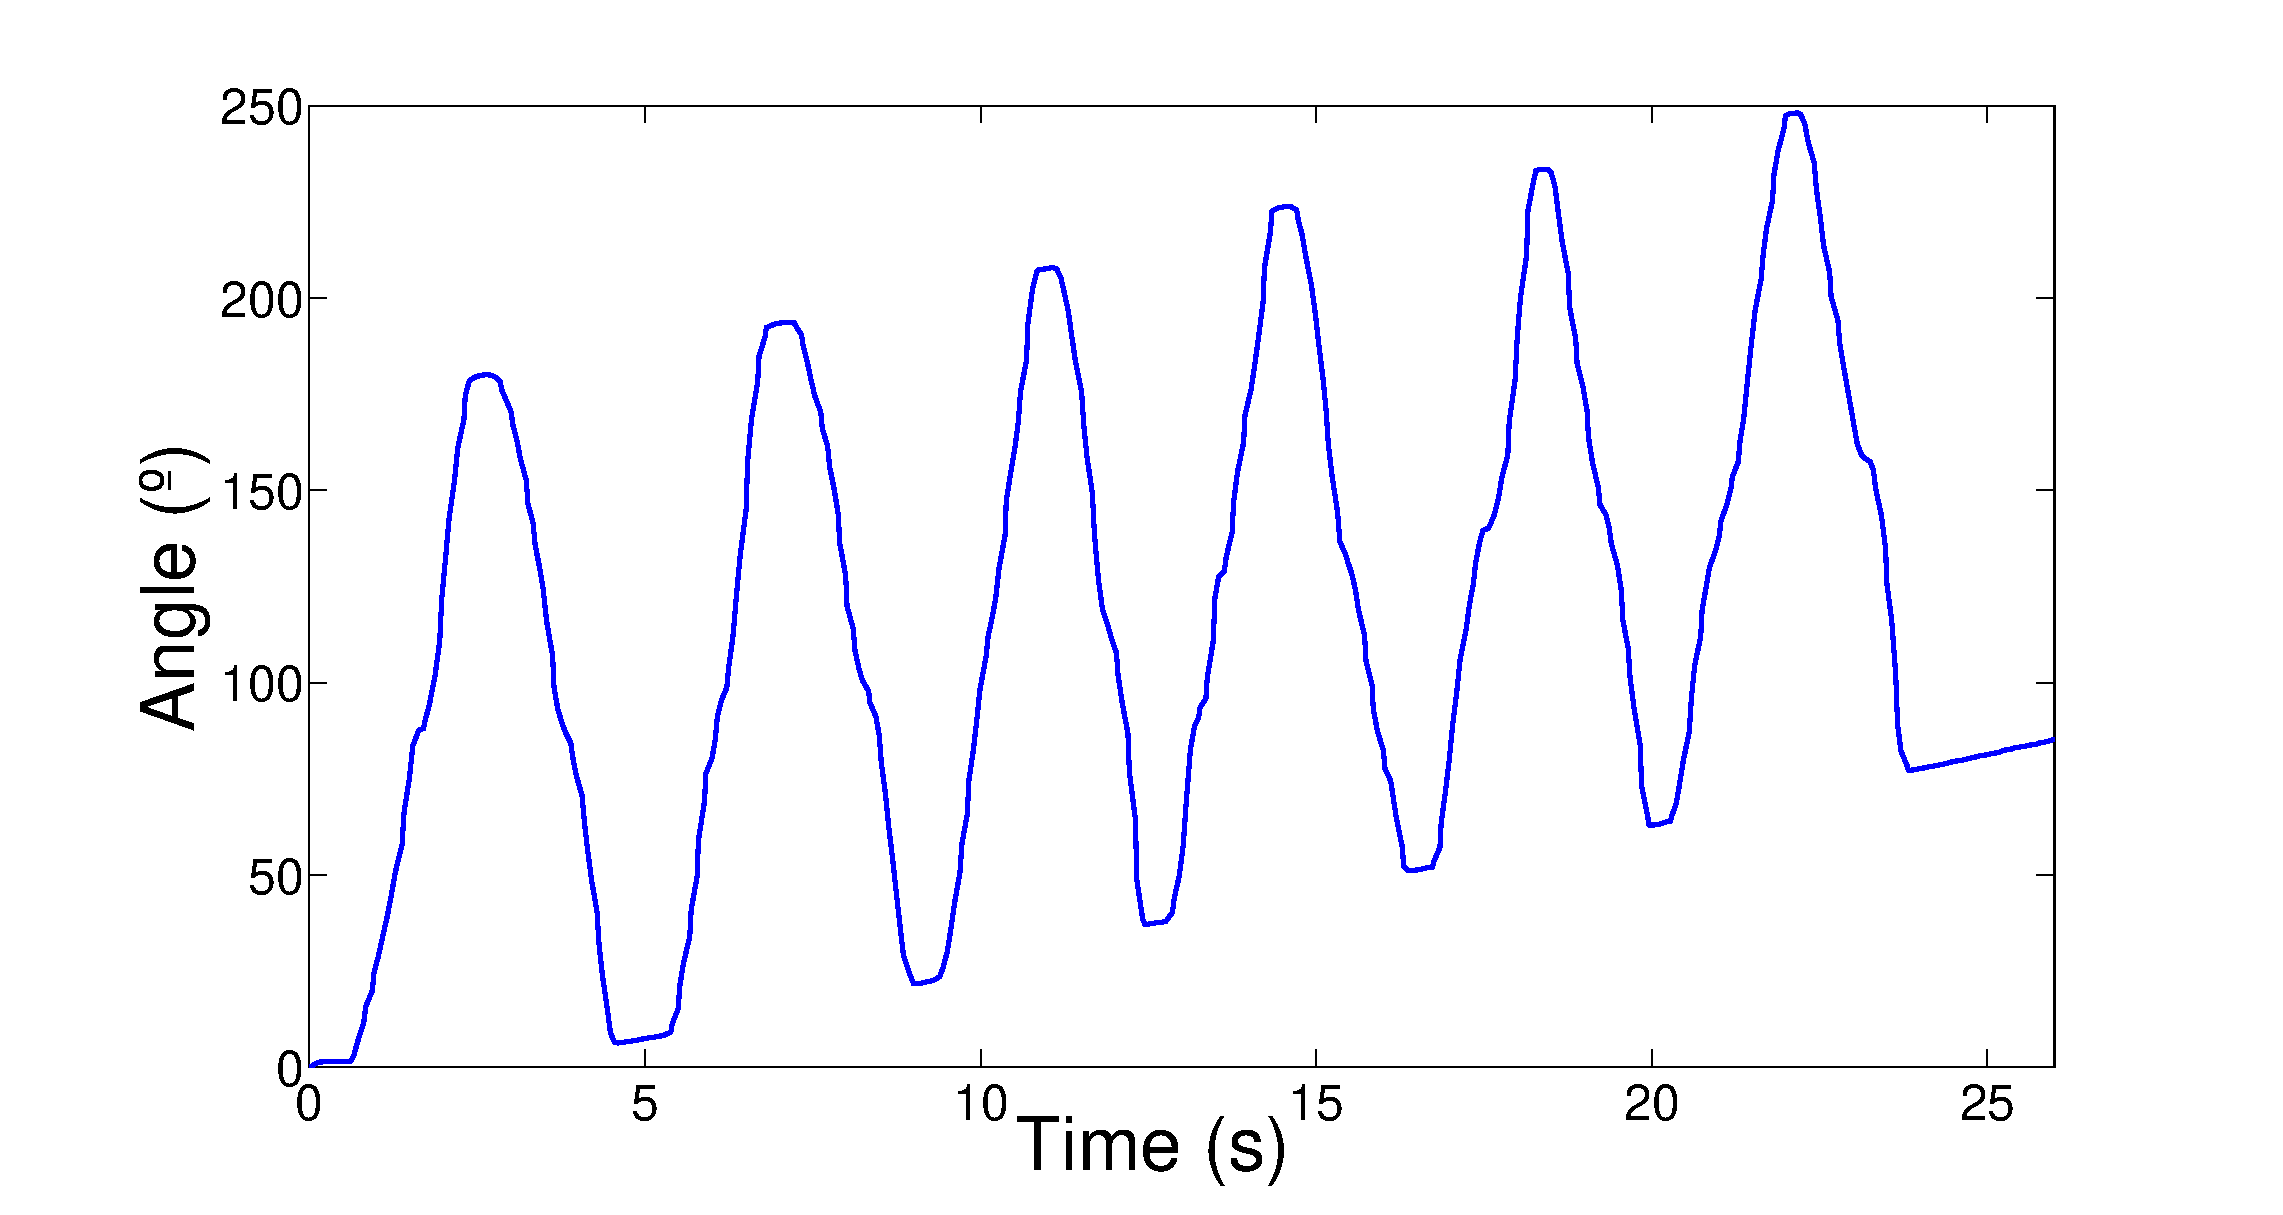
\includegraphics[width=0.7\textwidth]{figures/dynBiasEff.eps}
\caption{Effects of dynamic bias on the integrated gyroscope output signal.}
\label{fig:dynBiasEff}
\end{figure}


\subsection{Decomposition of gravity}
\indent We can use the projection of the Earth's gravity vector on the accelerometer's axes to estimate the orientation angle of the body frame with respect to the reference frame. In our case, this approach is used to compute the orientation angle of the thighs and shanks. Since only a biaxial accelerometer is available in the IMUs placed on these segments, we can only compute one of the two orientation angles (roll and pitch) which can be computed by means of this technique. We are interested on the angle of the segments defined in the XZ plane, that is, the angle around Y axis, which is defined as the pitch angle. The computation of the pitch will only be valid if the roll angle of the legs is close to zero. Since the legs move in the sagittal plane during gait, we can consider that the following expression will be valid to compute the pitch angle,

\begin{equation}
\label{eq:pitch_legs}
\theta_{k} = atan2(a_{z,k},a_{x,k})
\end{equation}

where $atan2$ is the quadrant-corrected arctangent function.

\subsection{Fusing the angular rate with the orientation angle observation computed with the accelerometer}
\subsubsection{The Kalman filter}
\label{subsubsec:kalman_filter}
\indent \indent The Kalman filter \cite{Kalman60}, \cite{Welch2001}, \cite{grewal_kalman_2008} is a set of mathematical equations that provides a means to estimate the state of a process minimizing the mean of the squared error. \\
\indent If we consider a time invariant linear continuous model:
\begin{gather}
\dot{\textbf{x}}(t)=\mbox{F}\textbf{x}(t)+\mbox{C}\textbf{u}(t)+\mbox{I}_{\mbox{\footnotesize n}}\textbf{w}(t)\\\nonumber
\textbf{z}(t)=\mbox{H}\textbf{x}(t)+\mbox{I}_{\mbox{\footnotesize q}}\textbf{v}(t)
\label{eq:contSystem}
\end{gather}
where,
\begin{itemize}
\item the operator $\dot{\mathbf{x}}$ denotes the first derivative of $\mathbf{x}$.
\item $\mathbf{x}(t)\in\mathbb{R}^{\mbox{\scriptsize n}}$ is the (n$\times$1) state vector including the n state variables that describe the system.
\item $\mathbf{z}(t)\in\mathbb{R}^{\mbox{\scriptsize q}}$ is the (q$\times$1) output vector including the q real observations (measurements) of the state variables of the process.
\item $\mathbf{u}(t)\in\mathbb{R}^{\mbox{\scriptsize p}}$ is the (p$\times$1) control vector including the p input control signals.
\item F is the (n$\times$n) state transition matrix, or simply the state matrix.
\item C is the (n$\times$p) input matrix.
\item H is the (q$\times$n) output matrix.
\item $\mbox{I}_{\mbox{\footnotesize n}}$ is the (n$\times$n) identity matrix.
\item $\mbox{I}_{\mbox{\footnotesize q}}$ is the (q$\times$q) identity matrix.
\item $\mathbf{w}(t)\in\mathbb{R}^{\mbox{\scriptsize n}}$ is the (n$\times$1) process noise vector.
\item $\mathbf{v}(t)\in\mathbb{R}^{\mbox{\scriptsize q}}$ is the (q$\times$1) observation noise vector.
\end{itemize}
In the absence of a control input we have:
\begin{gather}
\dot{\textbf{x}}(t)=\mbox{F}\textbf{x}(t)+\mbox{I}_{\mbox{\footnotesize n}}\textbf{w}(t)\\\nonumber
\textbf{z}(t)=\mbox{H}\textbf{x}(t)+\mbox{I}_{\mbox{\footnotesize q}}\textbf{v}(t)
\label{eq:contSystem2}
\end{gather}
If we apply the forward-Euler approximation:
\begin{equation}
\dot{x}(t)\simeq \frac{x(t+\mbox{dt})-x(t)}{\mbox{dt}}
\end{equation}
we get:
\begin{gather}
\frac{\textbf{x}(t+\mbox{dt})-\textbf{x}(t)}{\mbox{dt}}\simeq \mbox{F}\textbf{x}(t)+\mbox{I}_{\mbox{\footnotesize n}}\textbf{w}(t)\\\nonumber
\textbf{x}(t+\mbox{dt})\simeq \left[\mbox{F}\textbf{x}(t)+\mbox{I}_{\mbox{\footnotesize n}}\textbf{w}(t)\right]\mbox{dt}+\textbf{x}(t)\\\nonumber
\textbf{x}(t+\mbox{dt})\simeq \mbox{F}\textbf{x}(t)\mbox{dt}+\mbox{I}_{\mbox{\footnotesize n}}\textbf{w}(t)\mbox{dt}+\textbf{x}(t)\\\nonumber
\textbf{x}(t+\mbox{dt})\simeq \left[\mbox{F}\mbox{dt}+\mbox{I}_{\mbox{\footnotesize n}}\right]\textbf{x}(t)+\mbox{I}_{\mbox{\footnotesize n}}\textbf{w}(t)\mbox{dt}
\end{gather}
If we now discretize the model:
\begin{gather}
\textbf{x}_{k+1}=\left[\mbox{F}\mbox{dt}+\mbox{I}_{\mbox{\footnotesize n}}\right]\textbf{x}_k+\mbox{I}_{\mbox{\footnotesize n}}\mbox{dt}\textbf{w}_k\\\nonumber
\textbf{x}_{k+1}=\Phi\textbf{x}_{k}+\mbox{I}_{\mbox{\footnotesize n}}\mbox{dt}\textbf{w}_{k}\\\nonumber
\textbf{z}_{k}=\mbox{H}\textbf{x}_{k}+\mbox{I}_{\mbox{\footnotesize q}}\mathbf{v}_{k}
\end{gather}
or how it is usually represented:
\begin{equation}
\textbf{x}_{k}=\Phi\textbf{x}_{k-1}+\mbox{B}\textbf{w}_{k-1}
\label{eq:DiscreteSystem}
\end{equation}
\begin{equation}
\textbf{z}_{k}=\mbox{H}\textbf{x}_{k}+\mbox{I}_{\mbox{\footnotesize q}}\mathbf{v}_{k}
\label{eq:DiscreteSystem2}
\end{equation}
where,
\begin{itemize}
\item $\mathbf{x}\in\mathbb{R}^{\mbox{\scriptsize n}}$ is again the (n$\times$1) state vector of the linear dynamic system.
\item $\mathbf{z}\in\mathbb{R}^{\mbox{\scriptsize q}}$ is again the (q$\times$1) vector of observations.
\item $\Phi$ is now the (n$\times$n) state transition matrix of the discrete linear dynamic system.
\item H is again the (q$\times$n) measurement sensitivity matrix defining the linear relationship between the state of the dynamic system and measurements that can be made.
\item $\mbox{B}=\mbox{I}_{\footnotesize \mbox{n}}\mbox{dt}$, where dt is the sampling period.
\item $\mathbf{w}\in\mathbb{R}^{\mbox{\scriptsize n}}$ is again the (n$\times$1) process noise vector.
\item $\mathbf{v}\in\mathbb{R}^{\mbox{\scriptsize q}}$ is again the (q$\times$1) observation noise vector.
\end{itemize}
\indent \indent So, when applied to discrete signals, the Kalman filter aims to solve the problem of trying to estimate the state $\mbox{\textbf{x}}\in\mathbb{R}^{n}$ of a discrete-time controlled process that is defined by the model in equations (\ref{eq:DiscreteSystem}) and (\ref{eq:DiscreteSystem2}). In addition, $\textbf{w}_{k}$ and $\textbf{v}_{k}$ are assumed to be independent of each other, white, and with normal probability distributions
\begin{equation}
p(\textbf{w})\thicksim N(0,\mbox{Q})
\label{eq:ProbDistW}
\end{equation}
\begin{equation}
p(\textbf{v})\thicksim N(0,\mbox{R})
\label{eq:ProbDistV}
\end{equation}
where, in turn, Q and R are the process noise covariance and measurement noise covariance matrices respectively and can be considered to be invariant in practice.\\
\indent When deriving the equations for the Kalman filter, the goal is to find an equation that computes an a posteriori (updated/corrected with the measurement) state estimate $\hat{\textbf{x}}_{k}$ as a linear combination of an a priori (predicted) estimate $\hat{\textbf{x}}_{k}^{-}$ and a weighted difference between an actual measurement $\textbf{z}_{k}$ and a measurement prediction $\mbox{H}\hat{\textbf{x}}_{k}^{-}$,
\begin{equation}
\hat{\textbf{x}}_{k}=\hat{\textbf{x}}_{k}^{-}+\mbox{K}_{k}(\textbf{z}_{k}-H\hat{\textbf{x}}_{k}^{-}).
\label{eq:KalProcEst}
\end{equation}
The difference in (\ref{eq:KalProcEst}) is known as the measurement innovation, or the residual. The residual indicates the discordance between the predicted measurement $\mbox{H}\hat{\textbf{x}}_{k}^{-}$ and the actual measurement $\textbf{z}_{k}$.\\
\indent The matrix $\mbox{K}_{k}$ in (\ref{eq:KalProcEst}) is known as the Kalman gain and is chosen to be the gain that will minimize the a posteriori error covariance. Another way to see the weighting by $\mbox{K}_{k}$ is that as the measurement error covariance gets close to zero, the actual measurement $\textbf{z}_{k}$ is trusted more, while the predicted measurement $\mbox{H}\hat{\textbf{x}}_{k}^{-}$ is trusted less. Analogously, as the a priori estimate error covariance approaches zero the actual measurement is trusted less, while the predicted measurement is trusted more.\\
\indent The Kalman filter estimates a process by using a form of feedback control: the filter estimates the process state at some time and then obtains feedback in the form of noisy measurements. As such, the equations for the Kalman filter are divided into two groups: time update equations and measurement update equations.\\
\indent The time update equations can also be thought of as prediction equations, while the measurement update equations can be thought of as correction equations. If we assume $\Phi$, H, Q and R to be constant, the time update equations are as follows:
\begin{equation}
\hat{\textbf{x}}_{k}^{-}=\Phi\hat{\textbf{x}}_{k-1}^{-}
\label{eq:prioriProcEst}
\end{equation}
\begin{equation}
\mbox{P}_{k}^{-}=\Phi \mbox{P}_{k-1}\Phi^{T}+\mbox{Q}
\label{eq:prioriCov}
\end{equation}
while the measurement update equations are
\begin{equation}
\mbox{K}_{k}=\mbox{P}_{k}^{-}\mbox{H}^{T}(\mbox{H}\mbox{P}_{k}^{-}\mbox{H}^{T}+\mbox{R})^{-1}
\label{eq:KalGain}
\end{equation}
\begin{equation}
\hat{\textbf{x}}_{k}=\hat{\textbf{x}}_{k}^{-}+\mbox{K}_{k}(\textbf{z}_{k}-\mbox{H}\hat{\textbf{x}}_{k}^{-})
\label{eq:postProcEst}
\end{equation}
\begin{equation}
\mbox{P}_{k}=(\mbox{I}-\mbox{K}_{k}\mbox{H})\mbox{P}_{k}^{-}
\label{eq:postCov}
\end{equation}
where $\mbox{P}_{k}^{-}$ and $\mbox{P}_{k}$ are the a priori and a posteriori estimate error covariance respectively and $\mbox{K}_{k}$ is a factor known as the Kalman Gain.\\
\indent Consequently in order to build a computational algorithm the following steps must be implemented:
\begin{itemize}
\item Known parameters.
    \begin{enumerate}
    \item $\Phi$:   State transition matrix.
    \item H:  Measurement matrix.
    \item Q:  Process noise covariance matrix.
    \item R:  Measurement noise covariance matrix.
    \end{enumerate}
\item Computations.
    \begin{enumerate}
    \item Compute $\mbox{P}_{k}^{-}$ by substituting $\mbox{P}_{k-1}$, $\Phi$ and Q in (\ref{eq:prioriCov}).
    \item Compute $\mbox{K}_{k}$ by substituting $\mbox{P}_{k}^{-}$, H and R in (\ref{eq:KalGain}).
    \item Compute $\mbox{P}_{k}$ by substituting $\mbox{K}_{k}$ and $\mbox{P}_{k}^{-}$ in (\ref{eq:postCov}).
    \item Compute successive values of $\hat{\textbf{x}}_{k}$ (which is the output of the filter) recursively using (\ref{eq:prioriProcEst}), (\ref{eq:postProcEst}) and the computed values of $\mbox{K}_{k}$. Start with the given initial estimates $\hat{\textbf{x}}_0$ and $\mbox{P}_{0}$.
    \end{enumerate}
\end{itemize}

\indent Figure \ref{fig:StandardKalmanDiagram} shows the flow diagram of the standard approach of the Kalman filter without sensor fusion.
\begin{figure}[H]
\centering
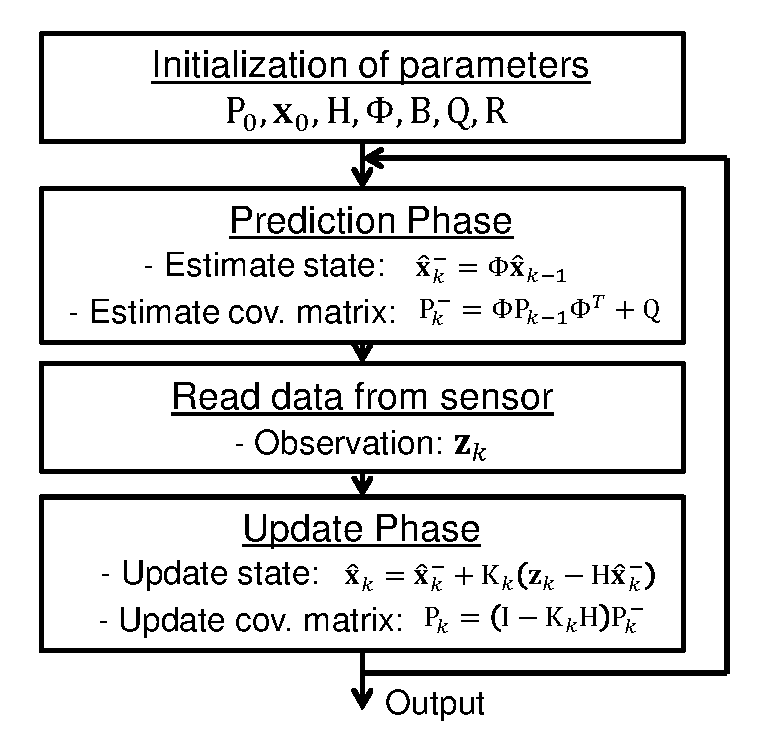
\includegraphics[width=0.6\textwidth]{figures/StandardKalmanDiagram.eps}
\caption{General diagram of the standard approach of the Kalman filter without sensor fusion.}
\label{fig:StandardKalmanDiagram}
\end{figure}

\subsubsection{The Kalman filter applied to orientation estimation}
\indent After this brief introduction to the basic theoretical fundamentals of the Kalman filter, we now explain how to employ it in a sensor fusion approach, and more specifically how to apply it to fuse the information coming from the two orientation estimation approaches explained to the moment.\\
\indent Let the state vector that we want to estimate be the following:
\begin{equation}
\mathbf{x}(t)=\left[
                \begin{array}{c}
                  \alpha(t) \\
                  \mbox{bias}(t) \\
                \end{array}
              \right]
\label{eq:kal_state}
\end{equation}
where $\alpha(t)$ is any of the orientation angles (roll, pitch or yaw), and bias(t) is the difference between the measured angular rate and the actual angular rate for $\alpha$.
\begin{equation}
\mbox{bias}(t)=\omega_{\mbox{\footnotesize meas}}(t)-\omega_{\mbox{\footnotesize actual}}(t)
\label{eq:kal_bias}
\end{equation}
Also, let $\mathbf{w}(t)=[w_{\alpha}(t)\;w_{bias}(t)]^{T}$, be the vector composed of the angle estimation noise and the angular rate bias noise respectively. The observation of the process, $\mathbf{z}(t)$ is the estimation of the angle computed using the accelerometer-magnetometer approach.
\begin{equation}
\mathbf{z}(t)=z(t)=\alpha(t)
\label{eq:Kal_fus_obs}
\end{equation}
We now proceed to obtain the expressions of the derivatives of the state variables:
\begin{equation}
\frac{\mbox{d}\alpha(t)}{\mbox{d}t}=\omega_{\mbox{\footnotesize actual}}(t)
\label{eq:Kal_fus_assum}
\end{equation}
knowing that $\omega_{\mbox{\footnotesize actual}}(t)=\omega_{\mbox{\footnotesize meas}}(t)-\mbox{bias}(t)$, i.e. the measured angular rate presents an offset with respect to its actual value:
\begin{equation}
\frac{\mbox{d}\alpha(t)}{\mbox{d}t}=\omega_{\mbox{\footnotesize meas}}(t)-\mbox{bias}(t)
\label{eq:Kal_fus_assum2}
\end{equation}
If we consider $\omega_{\mbox{\footnotesize meas}}(t)$ as a part of the process noise, $\omega_{\mbox{\footnotesize meas}}(t)=w_{\alpha}(t)$, we get:
\begin{equation}
\frac{\mbox{d}\alpha(t)}{\mbox{d}t}=-\mbox{bias}(t)+w_{\alpha}(t)
\label{eq:KalAngleDeriv}
\end{equation}
Thus, the first component of the process noise power, $w_{\alpha}(t)$ should be the variance of the angle signal computed with the accelerometer-magnetometer approach. \\ \\
\indent On the other hand, let the derivative of the second state variable, bias($t$), be the second component of the process noise:
\begin{equation}
\frac{\mbox{d}\mbox{bias}(t)}{\mbox{d}t}=w_{\mbox{\footnotesize bias}}(t)
\end{equation}
Then, the model of the system is as follows:
\begin{gather}
\mathbf{x}(t)=\left[
                \begin{array}{c}
                  \alpha(t) \\
                  \mbox{bias}(t) \\
                \end{array}
              \right];\nonumber\\
\frac{\mbox{d}\mathbf{x}(t)}{\mbox{d}t}=\frac{\mbox{d}}{\mbox{d}t}\left[
                                        \begin{array}{c}
                                          \alpha(t) \\
                                          \mbox{bias}(t) \\
                                        \end{array}
                                      \right]=\left[
                                                \begin{array}{cc}
                                                  0 & -1 \\
                                                  0 & 0 \\
                                                \end{array}
                                              \right]\left[
                                        \begin{array}{c}
                                          \alpha(t) \\
                                          \mbox{bias}(t) \\
                                        \end{array}
                                      \right]+\left[
                                                \begin{array}{cc}
                                                  1 & 0 \\
                                                  0 & 1 \\
                                                \end{array}
                                              \right]\left[
                                        \begin{array}{c}
                                          w_{\alpha}(t) \\
                                          w_{\mbox{\footnotesize bias}}(t) \\
                                        \end{array}
                                      \right];\nonumber\\
z(t)=\left[1\;0\right]\left[
                    \begin{array}{c}
                      \alpha(t) \\
                      \mbox{bias}(t) \\
                    \end{array}
                  \right]+v(t)
\label{eq:Kal_fus_System}
\end{gather}
If we now apply the approximations to discretize the system we get:
\begin{gather}
\mathbf{x}_{k+1}=\left[
                   \begin{array}{c}
                     \alpha_{k+1} \\
                     \mbox{bias}_{k+1} \\
                   \end{array}
                 \right]=\left[\left[
                           \begin{array}{cc}
                             1 & 0 \\
                             0 & 1 \\
                           \end{array}
                         \right]+\left[
                                  \begin{array}{cc}
                                    0 & \mbox{-dt} \\
                                    0 & 0 \\
                                   \end{array}\right]\right]\left[
                   \begin{array}{c}
                     \alpha_{k} \\
                     \mbox{bias}_{k} \\
                   \end{array}
                 \right]+\left[
                           \begin{array}{cc}
                             \mbox{dt} & 0 \\
                             0 & \mbox{dt} \\
                           \end{array}
                         \right]\left[
                   \begin{array}{c}
                     w_{\alpha,k} \\
                     w_{\mbox{\footnotesize bias},k} \\
                   \end{array}
                 \right];\nonumber\\
\mathbf{z}_{k+1}=\left[1\;0\right]\left[
                   \begin{array}{c}
                     \alpha_{k+1} \\
                     \mbox{bias}_{k+1} \\
                   \end{array}
                 \right]+v_{k+1}
\label{eq:Kal_fus_disc_system}
\end{gather}
or, equivalently:
\begin{gather}
\mathbf{x}_{k}=\left[
                   \begin{array}{c}
                     \alpha_{k} \\
                     \mbox{bias}_{k} \\
                   \end{array}
                 \right]=\left[
                           \begin{array}{cc}
                             1 & -\mbox{dt} \\
                             0 & 1 \\
                           \end{array}
                         \right]\left[
                   \begin{array}{c}
                     \alpha_{k-1} \\
                     \mbox{bias}_{k-1} \\
                   \end{array}
                 \right]+\left[
                           \begin{array}{cc}
                             \mbox{dt} & 0 \\
                             0 & \mbox{dt} \\
                           \end{array}
                         \right]\left[
                   \begin{array}{c}
                     w_{\alpha,k-1} \\
                     w_{\mbox{\footnotesize bias},k-1} \\
                   \end{array}
                 \right];\nonumber\\
\mathbf{z}_{k}=\left[1\;0\right]\left[
                   \begin{array}{c}
                     \alpha_{k} \\
                     \mbox{bias}_{k} \\
                   \end{array}
                 \right]+v_{k}
\label{eq:Kal_fus_disc_system2}
\end{gather}
Then, identifying terms, we have:
\begin{equation}
\Phi=\left[
       \begin{array}{cc}
         1 & -\mbox{dt} \\
         0 & 1 \\
       \end{array}
     \right],\quad \mbox{B}=\left[
                           \begin{array}{cc}
                             \mbox{dt} & 0 \\
                             0 & \mbox{dt} \\
                           \end{array}
                         \right],\quad \mbox{H}=\left[1\;0\right]
\label{eq:identified_filter_matrices}
\end{equation}

\indent Once we have defined the state equations of the discrete system, we repeat the equations of the Kalman filter and their order of application for the sake of clarity:
\begin{center}
\underline{PREDICTION EQUATIONS}
\end{center}
\vspace{-0.5cm}
\begin{equation}
\mathbf{\hat{x}}_{k}^{-}=\Phi\mathbf{\hat{x}}_{k-1}
\label{eq:Kal_fus_pred1}
\end{equation}
\begin{equation}
\mbox{P}_{k}^{-}=\Phi\mbox{P}_{k-1}\Phi^{T}+\mbox{Q}
\label{eq:Kal_fus_pred2}
\end{equation}
\begin{center}
\underline{UPDATE EQUATIONS}
\end{center}
\vspace{-0.5cm}
\begin{equation}
\mbox{K}_{k}=\frac{\mbox{P}_{k}^{-}\mbox{H}^{T}}{\mbox{H}\mbox{P}_{k}^{-}\mbox{H}^{T}+\mbox{R}}
\label{eq:Kalman_gain_update_phase}
\end{equation}
\begin{equation}
\mathbf{\hat{x}}_{k}=\mathbf{\hat{x}}_{k}^{-}+\mbox{K}_{k}(\mbox{z}_{k}-\mbox{H}\mathbf{\hat{x}}_{k}^{-})
\label{eq:state_vector_update_phase}
\end{equation}
\begin{equation}
\mbox{P}_{k}=(\mbox{I}-\mbox{K}_{k}\mbox{H})\mbox{P}_{k}^{-}
\label{eq:covariance_matrix_update_phase}
\end{equation}
where
\begin{itemize}
\item $\mathbf{\hat{x}}_{k}^{-}$ is the a priori state estimate.
\item $\mbox{P}_{k}^{-}$ is the a priori system covariance matrix.
\item $\mbox{Q}$ is the process noise covariance matrix and is defined as
\begin{equation}
\mbox{Q}=\left[
    \begin{array}{cc}
      \sigma_{\alpha} & 0 \\
      0 & \sigma_{\omega} \\
    \end{array}
  \right]
\label{eq:Kal_fus_proc_noise_cov_matrix}
\end{equation}
where $\sigma_{\alpha}$ is the variance of the angle computed with the acce\-le\-ro\-me\-ter-mag\-ne\-to\-me\-ter approach and $\sigma_{\omega}$ the variance of the angular rate measured by the gyroscope.
\item R, which in this case is a scalar, is the power of the observation noise and is defined as the variance of the accelerometer-magnetometer angle estimation ($\sigma_{\alpha}$).
\item $\mbox{K}_{k}$ is the Kalman filter gain.
\item $\mathbf{\hat{x}}_{k}$ is the a posteriori state estimate.
\item $\mbox{P}_{k}$ is the a posteriori system covariance matrix.
\end{itemize}
The reader may be wondering where exactly in the equations we have used the measured angular rate. Truth is that equations (\ref{eq:Kal_fus_pred1})-(\ref{eq:covariance_matrix_update_phase}) do not yet implement a sensor fusion approach as we are only using data coming from the accelerometer-magnetometer. The key of inserting sensor fusion to the system defined by these equations is to change the computation of the a priori prediction of the states $\mathbf{\hat{x}}_{k}^{-}$ as follows:
\begin{equation}
\mathbf{\hat{x}}_{k}^{-}=\left[
                           \begin{array}{c}
                             \alpha_{k}^{-} \\
                             \mbox{bias}_{k}^{-} \\
                           \end{array}
                         \right]=
\left[
                           \begin{array}{c}
                             \alpha_{k-1}+\left(\omega_{\mbox{\footnotesize meas},k}-\mbox{bias}_{k-1}\right)\mbox{dt} \\
                             \mbox{bias}_{k-1}\\
                           \end{array}
                         \right]
\label{eq:Kal_fus_real_system}
\end{equation}
This way, the a priori state estimate is being computed using information from both accelerometer-magnetometer and angular rate approaches.\\
\indent To end the explanation of the classical approach of the Kalman filter applied to fuse the information of the accelerometer-magnetometer and gyroscope, we include below the step by step operations that need to be carried
out by the complete algorithm:
\begin{enumerate}
\item Initialize the covariance matrix as a $2\times2$ identity matrix, $\mbox{P}=\mbox{I}_{2\times2}$.
\item Define the covariance matrix using equation (\ref{eq:Kal_fus_proc_noise_cov_matrix}). This matrix remains constant during the execution of the algorithm.
\item Define the measurement noise variance, $R$, which in this case is the variance of the accelerometer-magnetometer angle estimations, $R=\sigma_{\alpha}$. This value remains constant during the execution of the algorithm.
\item Define the state transition and the measurement matrices, $\Phi$ and H using equation (\ref{eq:identified_filter_matrices}).
\item Read data from accelerometer ($\mathbf{a}_{k}$), gyroscope ($\mathbf{\omega}_{k}$) and magnetometer ($\mathbf{h}_{k}$). \label{en:read_data}
\item Using $\textbf{a}_{k}$ and $\mathbf{h}_{k}$, compute the accelerometer-magnetometer angle estimation, $\alpha_{k}$, by applying any of the non-fusion orientation estimation methods explained within the previous subsections.
\item Compute the a priori estimation of the state vector using equation (\ref{eq:Kal_fus_real_system}).
\item Compute the a priori system covariance matrix using equation (\ref{eq:Kal_fus_pred2}).
\item Compute the Kalman gain using equation (\ref{eq:Kalman_gain_update_phase}), where $z_{k}=\alpha_{k}$.
\item Update the state vector using equation (\ref{eq:state_vector_update_phase}).
\item Update the system covariance matrix using equation (\ref{eq:covariance_matrix_update_phase}).
\item Return to step \ref{en:read_data}.
\end{enumerate}
\indent Figure \ref{fig:KalmanDiagramFusion} shows the flow diagram of the standard approach of the Kalman filter with sensor fusion.
\begin{figure}[H]
\centering
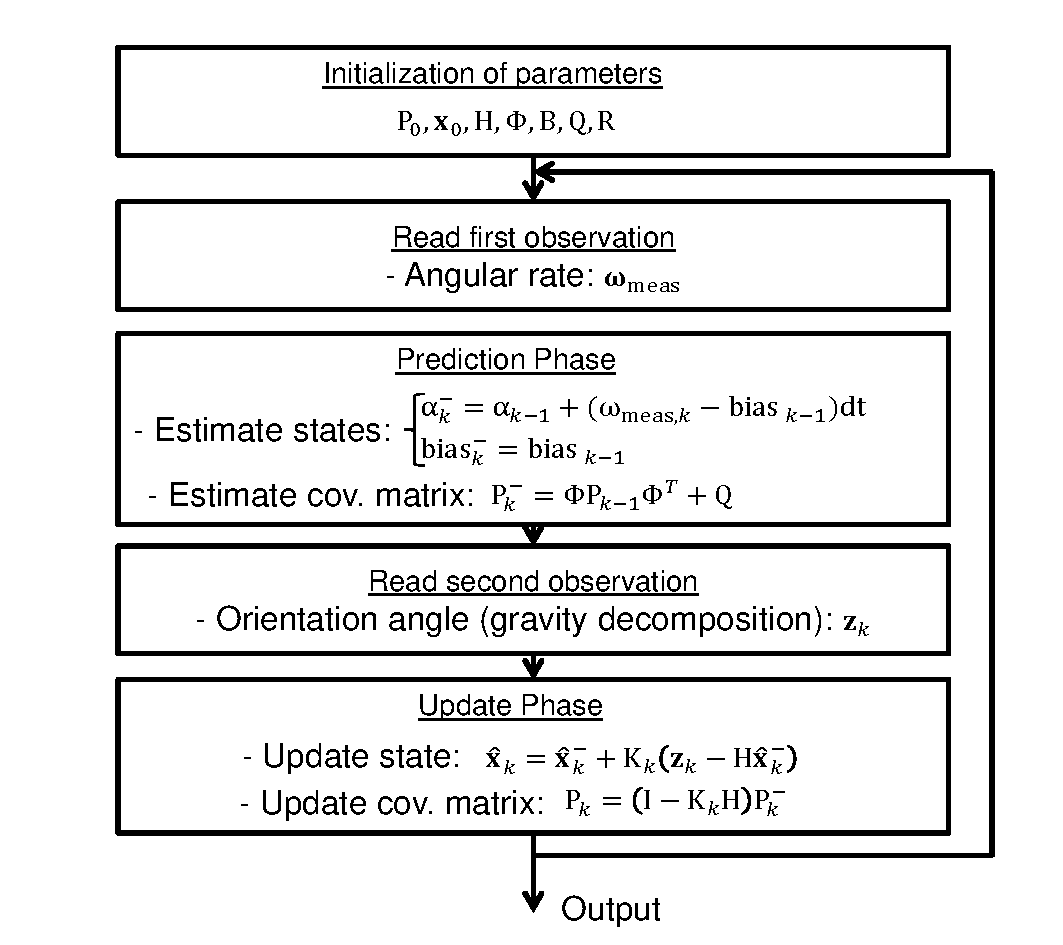
\includegraphics[width=0.8\textwidth]{figures/kalman_orientation_diag}
\caption{General diagram of the standard approach of the Kalman filter with sensor fusion.}
\label{fig:KalmanDiagramFusion}
\end{figure}

\section{Quaternion-based orientation determination}
\subsection{Using angular rate to compute orientation}
A way to compute the rate of change of the orientation of the Earth frame relative to the sensor frame is to compute the quaternion derivative $^{S}_{E}\dot{\textbf{q}}$, which is defined as follows,
\begin{equation}
\label{eq:quat_deriv}
^{S}_{E}\dot{\mathbf{q}} = \frac{1}{2}{^{S}_{E}\textbf{q}}\otimes{^{S}\boldsymbol{\omega}}
\end{equation}
where $^{S}_{E}\textbf{q}$ is the quaternion determining the orientation of the Earth frame relative to the sensor frame, $^{S}\boldsymbol{\omega} = \left[0\;\omega_{x}\;\omega_{y}\;\omega_{z}\right]$ is the measured angular rate vector in the sensor frame in quaternion form, and $\otimes$ is the quaternion (or Hamiltonian) product. \\
\indent Therefore, we can compute the orientation of the Earth frame relative to the sensor frame (computed from the angular rate) at time t  $^{S}_{E}\textbf{q}_{\omega,t}$ by simply numerically integrating the quaternion derivative in equation (\ref{eq:quat_deriv}).

\begin{equation}
\label{eq:quat_integration}
^{S}_{E}\mathbf{q}_{\omega,t} = ^{S}_{E}\mathbf{\hat{q}}_{t-1} + ^{S}_{E}\dot{\mathbf{q}}_{w,t}\Delta t
\end{equation}

where $^{S}_{E}\mathbf{\hat{q}}_{t-1}$ is the orientation quaternion estimated in $t-1$ by applying a sensor fusion algorithm (this will be later explained), and $\Delta t$ is the sampling frequency. So, if we plug equation (\ref{eq:quat_deriv}) into (\ref{eq:quat_integration}), we get

\begin{equation}
\label{eq:state_equations}
\begin{gathered}
\begin{multlined}
^{S}_{E}\mathbf{q}_{\omega,t} = \left[\hat{q}_{1,t-1}\;\hat{q}_{2,t-1}\;\hat{q}_{3,t-1}\;\hat{q}_{4,t-1}\right] + \frac{1}{2}\Delta t\left[\hat{q}_{1,t-1}\;\hat{q}_{2,t-1}\;\hat{q}_{3,t-1}\;\hat{q}_{4,t-1} \right]\otimes\left[0\;\omega_{x}\;\omega_{y}\;\omega_{z}\right] =\\ \noindent
= \left[\hat{q}_{1,t-1}\;\hat{q}_{2,t-1}\;\hat{q}_{3,t-1}\;\hat{q}_{4,t-1}\right] + \frac{1}{2}\Delta t\biggl[\underbrace{-\hat{q}_{2,t-1}\omega_{x}-\hat{q}_{3,t-1}\omega_{y}-\hat{q}_{4,t-1}\omega_{z}}_{y_{1'}}\\
\underbrace{\hat{q}_{1,t-1}\omega_{x}+\hat{q}_{3,t-1}\omega_{z}-\hat{q}_{4,t-1}\omega_{y}}_{y_{2'}}\;\underbrace{\hat{q}_{1,t-1}\omega_{y}-\hat{q}_{2,t-1}\omega_{z}+\hat{q}_{4,t-1}\omega_{x}}_{y_{3'}}\;\\
\underbrace{\hat{q}_{1,t-1}\omega_{z}+\hat{q}_{2,t-1}\omega_{y}-\hat{q}_{3,t-1}\omega_{x}}_{y_{4'}}\biggr]
\end{multlined}
\end{gathered}
\end{equation}

\subsection{Using acceleration and magnetic field to compute orientation}
Another possible way to compute the orientation is by using the accelerometer and the magnetometer measurements. The accelerometer measures the magnitude and direction of the Earth's gravitational field in addition to linear acceleration. The magnetometer measures as well the magnitude and direction of the Earth's magnetic field together with local magnetic flux and field perturbations. \\
\indent If the body is moving with quasi-static motion and the environment is magnetically stable, we can assume that the accelerometer will only measure the gravity and the magnetometer will only measure Earth's magnetic field. We will assume this in the following.\\
\indent In order to obtain a complete 9-DOF orientation estimate we need to combine both the accelerometer and the magnetometer as the accelerometer is not able to measure the orientation around the Z axis as it is parallel to the gravitational field. In some applications it is only necessary to measure pitch and/or roll, so there is no need for a magnetometer. However, for a quaternion-based solution we need both sensors as it is a 9-DOF estimation.\\
\indent Therefore, to estimate the complete orientation we can formulate an optimization problem where an orientation of the sensor $^{S}_{E}\dot{\mathbf{q}}$, is that which aligns a predefined reference direction of the field in the Earth frame, $^{E}\mathbf{\hat{d}}$, with the measured direction of the field in the sensor frame, $^{S}\mathbf{\hat{s}}$, using the quaternion rotation operation 

\begin{equation}
\label{eq:quat_rot}
^{E}\mathbf{v} = ^{E}_{S}\hat{\mathbf{q}}\otimes^{S}\mathbf{v}\otimes^{E}_{S}\hat{\mathbf{q}}
\end{equation}

where $^{E}\mathbf{v}$ and $^{S}\mathbf{v}$ represent the vector $\mathbf{v}$ measured in the Earth frame and the sensor frame respectively, and $^{E}_{S}\hat{\mathbf{q}}$ is the quaternion representing the orientation of the sensor frame with respect to the Earth frame. \\
\indent Hence, $^{E}_{S}\hat{\mathbf{q}}$ can be found as the solution of 

\begin{equation}
\label{eq:quat_opt_problem}
\min_{^{E}_{S}\hat{\mathbf{q}}\in\mathbb{R}^{4}}f\left(^{E}_{S}\hat{\mathbf{q}},^{E}\hat{\mathbf{d}},^{S}\hat{\mathbf{s}}\right)
\end{equation}

where 

\begin{equation}
\label{eq:quat_opt_func}
f\left(^{E}_{S}\hat{\mathbf{q}},^{E}\hat{\mathbf{d}},^{S}\hat{\mathbf{s}}\right) = ^{E}_{S}\hat{\mathbf{q}}^{*}\otimes^{E}\hat{\mathbf{d}}\otimes^{E}_{S}\hat{\mathbf{q}}-^{S}\hat{\mathbf{s}}
\end{equation}

In this case, we will use the gradient descent algorithm to optimize the function. The orientation quaternion at instant k+1 is computed applying

\begin{equation}
\label{eq:quat_gradient}
^{E}_{S}\hat{\mathbf{q}}_{k+1} = ^{E}_{S}\hat{\mathbf{q}}_{k}-\mu\frac{\nabla f\left(^{E}_{S}\hat{\mathbf{q}},^{E}\hat{\mathbf{d}},^{S}\hat{\mathbf{s}}\right)}{\left\Vert\nabla f\left(^{E}_{S}\hat{\mathbf{q}},^{E}\hat{\mathbf{d}},^{S}\hat{\mathbf{s}}\right)\right\Vert}
\end{equation}

where 

\begin{equation}
\label{eq:quat_nabla}
\nabla f\left(^{E}_{S}\hat{\mathbf{q}},^{E}\hat{\mathbf{d}},^{S}\hat{\mathbf{s}}\right) = J^{T}\left(^{E}_{S}\hat{\mathbf{q}}_{k},^{E}\hat{\mathbf{d}}\right)f\left(^{E}_{S}\hat{\mathbf{q}},^{E}\hat{\mathbf{d}},^{S}\hat{\mathbf{s}}\right)
\end{equation}

Where, in turn,

\begin{equation}
\label{eq:quat_opt_func_extended}
^{E}_{S}\hat{\mathbf{q}}^{*}\otimes^{E}\hat{\mathbf{d}}\otimes^{E}_{S}\hat{\mathbf{q}}-^{S}\hat{\mathbf{s}} = 
\left[\begin{array}{c}
	2d_{x}\left(\frac{1}{2} - q_{3}^{2} - q_{4}^{2}\right) + 2d_{x} + 2d_{y}\left(q_{1}q_{4}+q_{2}q_{3}\right) +2d_{z}\left(q_{2}q_{4}-q_{1}q_{3}\right) - s_{x} \\
	2d_{x}\left(q_{2}q_{3} - q_{1}q_{4}\right) + 2d_{y}\left(\frac{1}{2} - q_{2}^2 - q_{4}^2\right) + 2d_{z}\left(q_{1}q_{2} + q_{3}q_{4}\right) - s_{y} \\
	2d_{x}\left(q_{1}q_{3} + q_{2}q_{4}\right) + 2d_{y}\left(q_{3}q_{4} - q_{1}q_{2}\right) + 2d_{z}\left(\frac{1}{2} - q_{2}^2 - q_{3}^2\right) - s_{z}
\end{array}\right]
\end{equation}

As we aforementioned,

\begin{itemize}
\item $^{E}_{S}\hat{\mathbf{q}} = \left[q_{1}\: q_{2}\: q_{3}\: q_{4}\right]\rightarrow$ Estimated orientation quaternion.
\item $^{E}\hat{\mathbf{d}} = \left[0\: d_{x}\: d_{y}\: d_{z}\right]\rightarrow$ Predefined reference direction of the field in the Earth frame.
\item $^{S}\hat{\mathbf{s}} = \left[0\: s_{x}\: s_{y}\: s_{z}\right]\rightarrow$ Measured direction of the field in the sensor frame.
\end{itemize}

In our case, we have two reference vectors, the Earth's gravitational and magnetic field vectors. Therefore, we will use both to have a complete 9DOF orientation estimation. We will start by deriving the equations for the Earth's gravitational field and the accelerometer. For this case, $^{E}\hat{\mathbf{d}} = ^{E}\hat{\mathbf{g}} = \left[0\: 0\: 0\: 1\right]$ and $^{S}\hat{\mathbf{s}} = ^{S}\hat{\mathbf{a}} = \left[0\: a_{x}\: a_{y}\: a_{z}\right]$. Then, equation (\ref{eq:quat_opt_func_extended}) is reduced to,

\begin{equation}
\label{eq:quat_opt_func_reduced}
f\left(^{E}_{S}\hat{\mathbf{q}},^{E}\hat{\mathbf{g}},^{S}\hat{\mathbf{a}}\right) = ^{E}_{S}\hat{\mathbf{q}}^{*}\otimes^{E}\hat{\mathbf{g}}\otimes^{E}_{S}\hat{\mathbf{q}}-^{S}\hat{\mathbf{a}} = \left[\begin{array}{c}
														 \underbrace{2\left(q_{2}q_{4} - q_{1}q_{3}\right) - a_{x}}_{F_{1}} \\
														 \underbrace{2\left(q_{1}q_{2} + q_{3}q_{4}\right) - a_{y}}_{F_{2}} \\
														 \underbrace{2\left(\frac{1}{2}-q_{2}^2-q_{3}^2\right) - a_{z}}_{F_{3}}
														\end{array}\right]
\end{equation}

As it was shown in equation (\ref{eq:quat_nabla}),

\begin{equation}
\label{eq:quat_nabla2}
\nabla f\left(^{E}_{S}\hat{\mathbf{q}},^{E}\hat{\mathbf{g}},^{S}\hat{\mathbf{a}}\right) = J^{T}\left(^{E}_{S}\hat{\mathbf{q}}_{k},^{E}\hat{\mathbf{g}}\right)f\left(^{E}_{S}\hat{\mathbf{q}},^{E}\hat{\mathbf{g}},^{S}\hat{\mathbf{a}}\right)
\end{equation}

Hence, we are only missing the computation of the Jacobian $J\left(^{E}_{S}\hat{\mathbf{q}}_{k},^{E}\hat{\mathbf{g}}\right)$, which is carried out by applying the following equation,

\begin{equation}
\label{eq:quat_jacobian}
J\left(^{E}_{S}\hat{\mathbf{q}}_{k},^{E}\hat{\mathbf{g}}\right) = \left[\begin{array}{cccc}
																																				\frac{\partial F_{1}}{\partial q_{1}} & \frac{\partial F_{1}}{\partial q_{2}} & \frac{\partial F_{1}}{\partial q_{3}} & \frac{\partial F_{1}}{\partial q_{4}} \\
																																				\frac{\partial F_{2}}{\partial q_{1}} & \frac{\partial F_{2}}{\partial q_{2}} & \frac{\partial F_{2}}{\partial q_{3}} & \frac{\partial F_{2}}{\partial q_{4}} \\
																																				\frac{\partial F_{3}}{\partial q_{1}} & \frac{\partial F_{3}}{\partial q_{2}} & \frac{\partial F_{3}}{\partial q_3{}} & \frac{\partial F_{3}}{\partial q_{4}}
																																			\end{array}\right] =
																																			\left[\begin{array}{cccc}
																																			-2q_{3} &  2q_{4} & -2q_{1} &  2q_{2} \\
																																			 2q_{2} &  2q_{1} &  2q_{4} &  2q_{3} \\
																																			      0 & -4q_{2} & -4q_{3} &       0
																																			\end{array}\right]
\end{equation}

We are now done with the accelerometer part, let's continue with the magnetometer which is going to provide the Yaw angle which can not be computed with the accelerometer. For the magnetometer, $^{E}\hat{\mathbf{d}} = ^{E}\hat{\mathbf{b}} = \left[0\: b_{x}\: 0\: b_{z}\right]$ and $^{S}\hat{\mathbf{s}} = ^{S}\hat{\mathbf{h}} = \left[0\: h_{x}\: h_{y}\: h_{z}\right]$.

\begin{equation}
\label{eq:quat_opt_func_reduced_mag}
f\left(^{E}_{S}\hat{\mathbf{q}},^{E}\hat{\mathbf{b}},^{S}\hat{\mathbf{h}}\right) = {^{E}_{S}\hat{\mathbf{q}}^{*}}\,\otimes\, {^{E}\hat{\mathbf{b}}}\,\otimes\, {^{E}_{S}\hat{\mathbf{q}}}-^{S}\hat{\mathbf{h}} = \left[\begin{array}{c}
														 \underbrace{2b_{x}\left(\frac{1}{2} - q_{3}^2-q_{4}^2\right) + 2b_{z}\left(q_{2}q_{4} - q_{1}q_{3}\right)- h_{x}}_{F_{4}} \\
														 \underbrace{2b_{x}\left(q_{2}q_{3} - q_{1}q_{4}\right) + 2b_{z}\left(q_{1}q_{2} + q_{3}q_{4}\right) - h_{y}}_{F_{5}} \\
														 \underbrace{2b_{x}\left(q_{1}q_{3} + q_{2}q_{4}\right) + 2b_{z}\left(\frac{1}{2} - q_{2}^2 - q_{3}^2\right)- h_{z}}_{F_{6}}
														\end{array}\right]
\end{equation}

Analogously as in equation (\ref{eq:quat_jacobian}),

\begin{equation}
\label{eq:quat_jacobian_mag}
\begin{gathered}
\begin{multlined}
J\left(^{E}_{S}\hat{\mathbf{q}}_{k},^{E}\hat{\mathbf{b}}\right) = \left[\begin{array}{cccc}
																																				\frac{\partial F_{4}}{\partial q_{1}} & \frac{\partial F_{4}}{\partial q_{2}} & \frac{\partial F_{4}}{\partial q_{3}} & \frac{\partial F_{4}}{\partial q_{4}} \\
																																				\frac{\partial F_{5}}{\partial q_{1}} & \frac{\partial F_{5}}{\partial q_{2}} & \frac{\partial F_{5}}{\partial q_{3}} & \frac{\partial F_{5}}{\partial q_{4}} \\
																																				\frac{\partial F_{6}}{\partial q_{1}} & \frac{\partial F_{6}}{\partial q_{2}} & \frac{\partial F_{6}}{\partial q_3{}} & \frac{\partial F_{6}}{\partial q_{4}}
																																			\end{array}\right] = \\
																																			= \left[\begin{array}{cccc}
																																			-2b_{z}q_{3} &  2b_{z}q_{4} & -2b_{z}q_{1} &  2b_{z}q_{2} \\
																																			-2b_{x}q_{4} + 2b_{z}q_{2} &  2b_{x}q_{3} + 2b_{z}q_{1} &  2b_{x}q_{2} + 2b_{z}q_{4} & -2b_{x}q_{1} + 2b_{z}q_{3} \\
																																			 2b_{x}q_{3} & 2b_{x}q_{4} - 4b_{z}q_{2} & 2b_{x}q_{1} - 4b_{z}q_{3} &  2b_{x}q_{2}
																																			\end{array}\right]
\end{multlined}
\end{gathered}
\end{equation}

So, finally, if we put everything together, these are the equations that need to be implemented to compute the orientation quaternion using accelerometer and magnetometer data,

\begin{gather}
\label{eq:quat_gradient_final}
^{E}_{S}\hat{\mathbf{q}}_{k+1} = {^{E}_{S}\hat{\mathbf{q}}_{k}}-\mu\frac{\nabla f\left(^{E}_{S}\hat{\mathbf{q}},^{E}\hat{\mathbf{gb}},^{S}\hat{\mathbf{ah}}\right)}{\left\Vert\nabla f\left(^{E}_{S}\hat{\mathbf{q}},^{E}\hat{\mathbf{gb}},^{S}\hat{\mathbf{ah}}\right)\right\Vert} \\
\nabla f\left(^{E}_{S}\hat{\mathbf{q}},^{E}\hat{\mathbf{gb}},^{S}\hat{\mathbf{ah}}\right) = J^{T}\left(^{E}_{S}\hat{\mathbf{q}}_{k},^{E}\hat{\mathbf{gb}}\right)f\left(^{E}_{S}\hat{\mathbf{q}},^{E}\hat{\mathbf{ah}},^{S}\hat{\mathbf{s}}\right) \\
\label{eq:quat_function_final}
f\left(^{E}_{S}\hat{\mathbf{q}},^{E}\hat{\mathbf{ah}},^{S}\hat{\mathbf{s}}\right) = \left[\begin{array}{c}
																																										 2\left(q_{2}q_{4} - q_{1}q_{3}\right) - a_{x} \\
																																										 2\left(q_{1}q_{2} + q_{3}q_{4}\right) - a_{y} \\
																																										 2\left(\frac{1}{2}-q_{2}^2-q_{3}^2\right) - a_{z} \\
																																										 2b_{x}\left(\frac{1}{2} - q_{3}^2-q_{4}^2\right) + 2b_{z}\left(q_{2}q_{4} - q_{1}q_{3}\right)- h_{x} \\
																																										 2b_{x}\left(q_{2}q_{3} - q_{1}q_{4}\right) + 2b_{z}\left(q_{1}q_{2} + q_{3}q_{4}\right) - h_{y} \\
																																										 2b_{x}\left(q_{1}q_{3} + q_{2}q_{4}\right) + 2b_{z}\left(\frac{1}{2} - q_{2}^2 - q_{3}^2\right)- h_{z}
																																										\end{array}\right] 
\end{gather}
\begin{gather}
\label{eq:final_Jacobian}
\begin{gathered}
\begin{multlined}																																							
J\left(^{E}_{S}\hat{\mathbf{q}}_{k},^{E}\hat{\mathbf{gb}}\right) = \left[\begin{array}{cccc}
																																				\frac{\partial F_{1}}{\partial q_{1}} & \frac{\partial F_{1}}{\partial q_{2}} & \frac{\partial F_{1}}{\partial q_{3}} & \frac{\partial F_{1}}{\partial q_{4}} \\
																																				\frac{\partial F_{2}}{\partial q_{1}} & \frac{\partial F_{2}}{\partial q_{2}} & \frac{\partial F_{2}}{\partial q_{3}} & \frac{\partial F_{2}}{\partial q_{4}} \\
																																				\frac{\partial F_{3}}{\partial q_{1}} & \frac{\partial F_{3}}{\partial q_{2}} & \frac{\partial F_{3}}{\partial q_3{}} & \frac{\partial F_{3}}{\partial q_{4}} \\
																																				\frac{\partial F_{4}}{\partial q_{1}} & \frac{\partial F_{4}}{\partial q_{2}} & \frac{\partial F_{4}}{\partial q_{3}} & \frac{\partial F_{4}}{\partial q_{4}} \\
																																				\frac{\partial F_{5}}{\partial q_{1}} & \frac{\partial F_{5}}{\partial q_{2}} & \frac{\partial F_{5}}{\partial q_{3}} & \frac{\partial F_{5}}{\partial q_{4}} \\
																																				\frac{\partial F_{6}}{\partial q_{1}} & \frac{\partial F_{6}}{\partial q_{2}} & \frac{\partial F_{6}}{\partial q_3{}} & \frac{\partial F_{6}}{\partial q_{4}}
																																			\end{array}\right] =\\ 
																																			 = \left[\begin{array}{cccc}
																																			-2q_{3} &  2q_{4} & -2q_{1} &  2q_{2} \\
																																			 2q_{2} &  2q_{1} &  2q_{4} &  2q_{3} \\
																																			      0 & -4q_{2} & -4q_{3} &       0 \\
																																			-2b_{z}q_{3} &  2b_{z}q_{4} & -2b_{z}q_{1} &  2b_{z}q_{2} \\
																																			-2b_{x}q_{4} + 2b_{z}q_{2} &  2b_{x}q_{3} + 2b_{z}q_{1} &  2b_{x}q_{2} + 2b_{z}q_{4} & -2b_{x}q_{1} + 2b_{z}q_{3} \\
																																			 2b_{x}q_{3} & 2b_{x}q_{4} - 4b_{z}q_{2} & 2b_{x}q_{1} - 4b_{z}q_{3} &  2b_{x}q_{2}
																																			\end{array}\right]
\end{multlined}
\end{gathered}
\end{gather}

The routine implementing the process above should be structured as follows for every instant $k$,

\begin{enumerate}[(i)]
\item Read the orientation quaternion for instant $k-1$, $^{E}_{S}\hat{\mathbf{q}}_{k-1}$.
\item Read the data from the accelerometer and the magnetometer for instant $k$. We then have $a_{x,k}\, a_{y,k}\, a_{z,k}\, h_{x,k}\, h_{y,k}$ and $h_{z,k}$.
\item Compute the Jacobian in equation (\ref{eq:final_Jacobian}) knowing that, 
	\begin{gather}
		\mathbf{m} = {^{E}_{S}\hat{\mathbf{q}}_{k-1}}\otimes \left[0\: h_{x,k}\: h_{y,k}\: h_{z,k}\right]\otimes {^{E}_{S}\hat{\mathbf{q}}_{k-1}^{*}} \\
		b_{x} = \sqrt{m_{2}^2+m_{3}^2} \\
		b_{z} = m_{4}
	\end{gather}
\item Compute the expression of $f\left(^{E}_{S}\hat{\mathbf{q}},^{E}\hat{\mathbf{ah}},^{S}\hat{\mathbf{s}}\right)$ in (\ref{eq:quat_function_final}).
\item Substitute the value of the expressions computed in the two previous steps in equation (\ref{eq:quat_gradient_final}) to compute the orientation quaternion for instant $k$, $^{E}_{S}\hat{\mathbf{q}}_{k}$.
\end{enumerate}

\subsection{Fusing the orientation quaternions computed with the angular rate and the acceleration and magnetic field}
\label{subsec:sensor_fusion}
\indent \indent In the previous two sections we have explained how to compute the orientation quaternion using two different approaches. The first one is based on the numerical integration of the angular rate. This approach would be perfect in an ideal situation in which there was no noise at the output of the gyroscope and no bias time drift. The second approach is based on the computation of the orientation of the gravity and the Earth's magnetic field vectors measured in the sensor frame with respect to their known reference value in the Earth's frame. This approach, as it was aforementioned is only valid if the body is measuring with negligible linear acceleration (i.e. low intensity motion) and/or there are not magnetic distortions nearby the sensors. \\
\indent It is clear then, that none of the two approaches can be used solely to compute an accurate orientation estimate. Therefore, we can apply a fusion scheme to fuse both approaches. The Extended Kalman Filter is a well known solution to carry out the sensor fusion. 

\subsubsection{The Extended Kalman Filter}
\label{subsubsec:extended_kalman_filter}

The Extended Kalman Filter is used when the process to be estimated and (or) the measurement relationship to the process is non-linear. A solution to the non-linearity is to linearize about the current mean and covariance. Let us assume that our process again has a state vector $\mathbb{R}^{n}$, but that the process is now governed by the non-linear stochastic difference equation,

\begin{equation}
x_{k}=f\left(x_{k-1},u_{k-1},w_{k-1}\right)
\label{eq:ekf_definition_1}
\end{equation}

with a measurement $z\in\mathbb{R}^{m}$,

\begin{equation}
z_{k} = h\left(x_{k},v_{k}\right)
\label{eq:ekf_definition_2}
\end{equation}

where the random variables $w_{k}$ and $v_{k}$ again represent the process and measurement noise. In this case, the non-linear function $f$ in the difference equation (\ref{eq:ekf_definition_1}) relates the state at the previous time step $k-1$ to the state at the current time step $k$. It includes as parameters any driving funciton $u_{k-1}$ and the zero-mean process noise $w_{k}$. The non-linear function $h$ in the measurement equation (\ref{eq:ekf_dfinition_2}) relates the state $x_{k}$ to the measurement $z_{k}$.\\

\indent In practice one does not know the individual values of the noise $w_{k}$ and $v_{k}$ at each time step. However, one can approximate the state and measurement vector without them as,

\begin{equation}
\bar{x}_{k}=f\left(\hat{x}_{k-1},u_{k-1},0\right)
\label{eq:ekf_definition_3}
\end{equation}

and 

\begin{equation}
\bar{z}_{k}=h\left(\bar{x}_{k},0\right)
\label{eq:ekf_definition_4}
\end{equation}

where $\hat{x}_{k}$ is some a posteriori estimate of the state from the previous time step k.\\

\indent To estimate a process with non-linear difference and measurement relationships, we begin by writing new governing equations that linearize an estimate about (\ref{eq:ekf_definition_3}) and (\ref{eq:ekf_definition_4}),

\begin{equation}
x_{k}\approx\bar{x}_{k}+A(x_{k-1}-\hat{x}_{k-1})+Ww_{k_1}
\label{eq:ekf_definition_5}
\end{equation}
\begin{equation}
z_{k}\approx\bar{z}_{k}+H(x_{k}-\bar{x}_{k})+Vv_{k}
\label{eq:ekf_definition_6}
\end{equation}

where,

\begin{itemize}
\item $x{k}$ and $z_{k}$ are the actual state and measurement vectors.
\item $\bar{x}_{k}$ and $\bar{z}_{k}$ are the approximate state and measurement vectors from (\ref{eq:ekf_definition_3}) and (\ref{eq:ekf_definition_4}).
\item The random variables $w_{k}$ and $v_{k}$ represent the process and measurement noise as in (\ref{eq:ekf_definition_1}) and (\ref{eq:ekf_definition_4}).
\item $A$ is the Jacobian matrix of partial derivatives of $f$ with respect to $x$, that is,
\begin{equation}
A_{[i,j]}=\frac{\partial f_{[i]}}{\partial x_{[j]}}\left(\hat{x}_{k-1},u_{k-1},0\right)
\label{eq:jacobian_matrix_A}
\end{equation}
\item $W$ is the Jacobian matrix of partial derivatives of $f$ with respect to $w$,
\begin{equation}
W_{[i,j]}=\frac{\partial f_{[i]}}{\partial w_{[j]}}\left(\hat{x}_{k-1},u_{k-1},0\right)
\label{eq:jacobian_matrix_W}
\end{equation}
\item $H$ is the Jacobian matrix of partial derivatives of $h$ with respect to $x$,
\begin{equation}
H_{[i,j]}=\frac{\partial h_{[i]}}{\partial x_{[j]}}\left(\bar{x}_{k},0\right)
\label{eq:jacobian_matrix_H}
\end{equation}
\item $V$ is the Jacobian of partial derivatives of $h$ with respect to $v$,
\begin{equation}
V_{[i,j]}=\frac{\partial h_{[i]}}{\partial v_{[j]}}\left(\bar{x}_{k},0\right)
\label{eq:jacobian_matrix_V}
\end{equation}
\end{itemize}

We can now define a new notation for the prediction error,

\begin{equation}
\bar{e}_{x_{k}}\equiv x_{k}-\bar{x}_{k}
\label{eq:ekf_state_error}
\end{equation}

and the measurement residual,

\begin{equation}
\bar{e}_{z_{k}}\equiv z_{k}-\bar{z}_{k}
\label{eq:ekf_meas_error}
\end{equation}

We can redefine these equations as,

\begin{equation}
\bar{e}_{x_{k}}\equiv A\left(x_{k-1}-\hat{x}_{k-1}\right)+\epsilon_{k}
\label{eq:ekf_state_error_2}
\end{equation}

\begin{equation}
\bar{e}_{z_{k}}\equiv H\bar{e}_{x_{k}} + \eta_{k}
\label{eq:ekf_meas_error_2}
\end{equation}

where $\epsilon_{k}$ and $\eta_{k}$ represent new independent random variables having zero mean and covariance matrices $QWW^{T}$ and $VRV^{T}$, with $Q$ and $R$ equal to the ones used in the standard Kalman filter.\\

In the end, we can compute the state estimate by applying the following equation,

\begin{equation}
\hat{x}_{k} = \bar{x}_{k}+K_{k}\left(z_{k}-\bar{z}_{k}\right)
\label{eq:ekf_state_correction}
\end{equation}

The complete set of EKF equations is shown below. Note that $\bar{x}_{k}$ has been substituted by $\hat{x}_{k}^{-}$ to remain consistent with the notation used in the standard Kalman Filter definition, and that the Jacobians $A, W, H$ and $V$ have the subscript $k$ to reinforce the notion that they are different at each time step.

\begin{itemize}
\item Time update equations:
\begin{equation}
\hat{x}_{k}^{-}=f\left(\hat{x}_{k-1},u_{k-1},0\right)
\label{eq:ekf_final_eq_1}
\end{equation}
\begin{equation}
\hat{P}_{k}^{-}=A_{k}P_{k-1}A_{k}^{T}+W_{k}Q_{k-1}W_{k}^{T}
\label{eq:ekf_final_eq_2}
\end{equation}
\item Measurement update equations:
\begin{equation}
K_{k}=P_{k}^{-}H_{k}^{T}\left(H_{k}P_{k}^{-}H_{k}^{T}+V_{k}R_{k}V_{k}^{T}\right)^{-1}
\label{eq:ekf_final_eq_3}
\end{equation}
\begin{equation}
\hat{x}_{k}=\hat{x}_{k}^{-}+K_{k}\left(z_{k}-h\left(\hat{x}_{k}^{-},0\right)\right)
\label{eq:ekf_final_eq_4}
\end{equation}
\begin{equation}
P_{k}=\left(I-K_{k}H_{k}\right)P_{k}^{-}
\label{eq:ekf_final_eq_5}
\end{equation}
\end{itemize}

\subsubsection{The Extended Kalman Filter applied to orientation estimation}
\label{subsubsec:ekf_orientation}
\indent The quaternion fusion is done by first defining the equations governing the process that we want to estimate. In our case, the state vector will be $^{S}_{E}\mathbf{q}_{t} = \left[q_{1} q_{2} q_{3} q_{4}\right]$ and the function $f$ is defined by equation \ref{eq:state_equations},

\begin{equation}
\label{eq:state_equations}
\begin{gathered}
\begin{multlined}
^{S}_{E}\mathbf{q}_{\omega,k} = \left[\hat{q}_{1,k-1}\;\hat{q}_{2,k-1}\;\hat{q}_{3,k-1}\;\hat{q}_{4,k-1}\right] + \frac{1}{2}\Delta t\left[\hat{q}_{1,k-1}\;\hat{q}_{2,k-1}\;\hat{q}_{3,k-1}\;\hat{q}_{4,k-1} \right]\otimes\left[0\;\omega_{x}\;\omega_{y}\;\omega_{z}\right] =\\ \noindent
= \left[\hat{q}_{1,k-1}\;\hat{q}_{2,k-1}\;\hat{q}_{3,k-1}\;\hat{q}_{4,k-1}\right] + \frac{1}{2}\Delta t\biggl[\underbrace{-\hat{q}_{2,k-1}\omega_{x}-\hat{q}_{3,k-1}\omega_{y}-\hat{q}_{4,k-1}\omega_{z}}_{y_{1'}}\\
\underbrace{\hat{q}_{1,k-1}\omega_{x}+\hat{q}_{3,k-1}\omega_{z}-\hat{q}_{4,k-1}\omega_{y}}_{y_{2'}}\;\underbrace{\hat{q}_{1,k-1}\omega_{y}-\hat{q}_{2,k-1}\omega_{z}+\hat{q}_{4,k-1}\omega_{x}}_{y_{3'}}\;\\
\underbrace{\hat{q}_{1,k-1}\omega_{z}+\hat{q}_{2,k-1}\omega_{y}-\hat{q}_{3,k-1}\omega_{x}}_{y_{4'}}\biggr]
\end{multlined}
\end{gathered}
\end{equation}

\begin{gather}
y_{1}=\hat{q}_{1,k-1}+y'_{1} = y_{1}=\hat{q}_{1,k-1}-\hat{q}_{2,k-1}\omega_{x}-\hat{q}_{3,k-1}\omega_{y}-\hat{q}_{4,k-1}\omega_{z}  \\ \nonumber
y_{2}=\hat{q}_{2,k-1}+y'_{2} = \hat{q}_{2,k-1} + \hat{q}_{1,k-1}\omega_{x}+\hat{q}_{3,k-1}\omega_{z}-\hat{q}_{4,k-1}\omega_{y} \\\nonumber
y_{3}=\hat{q}_{3,k-1}+y'_{3} = \hat{q}_{3,k-1} + \hat{q}_{1,k-1}\omega_{y}-\hat{q}_{2,k-1}\omega_{z}+\hat{q}_{4,k-1}\omega_{x} \\\nonumber
y_{4}=\hat{q}_{4,k-1}+y'_{4} = \hat{q}_{4,k-1} + \hat{q}_{1,k-1}\omega_{z}+\hat{q}_{2,k-1}\omega_{y}-\hat{q}_{3,k-1}\omega_{x}
\end{gather}

The measurement is given by the orientation quaternion computed using the acceleration and the magnetic field. Therefore, since the state vector is also composed of the orientation quaternion, the relationship between the state and the measurement is linear and the matrix $H$ is simply a $4\times4$ identity matrix.\\
\indent The matrix $A_{k}$ is computed applying equation (\ref{eq:jacobian_matrix_A}) which gives,

\begin{equation}
A_{k}=\left[\begin{array}{cccc}
			\frac{\partial y_{1,k}}{\partial} & \frac{\partial y_{1,k}}{\partial} & \frac{\partial y_{1,k}}{\partial} & \frac{\partial y_{1,k}}{\partial}
			\end{array}\right]
\label{eq:A_final}
\end{equation}